% =====================================================================
% CAPITOLO 3 — stesura della candidata, con le correzioni dell'8 settembre.
%
% ATTENZIONE, e' ISS-110: questo NON e' `Cap3.tex` del repository. Prima
% della consegna va deciso quale copia sia quella buona.
%
% CHE COSA E' CAMBIATO, in ordine di importanza:
%
% 1. §3.3.4 — il paragrafo sull'fps misurato e' stato SPOSTATO. Era finito
%    dopo «Rappresentazione scheletrica grezza», ma comincia con «Questa
%    uniformazione», e l'antecedente stava due paragrafi prima. Ora segue
%    direttamente la frase su Delta t = 1/fps.
%
% 2. §3.4.1 — tabella dell'autocorrelazione RIFATTA su feature_v4.csv
%    (`pipeline/autocorrelazione.py`). Tolta «Energia del corpo»: era la
%    grandezza che §3.3.4 dichiara di aver eliminato perche' sommava
%    quadrati con unita' diverse, e usarla come prova era una
%    contraddizione interna. E l'affermazione «valori superiori a 0,9» era
%    FALSA: percorso vale 0,840 e discesa 0,785. Sostituita con
%    un'affermazione di separazione, che e' piu' forte e vera.
%
% 3. §3.4 — il fattore 18*sqrt(2) non e' una costante: varia fra 20,4 e
%    27,8 alle cadenze reali.
%
% 4. §3.8 — aggiunto il paragrafo «Il confine, e che cosa se ne fa»: una
%    finestra con l'evento sotto soglia diventava un negativo pulito, e
%    nessuno lo dichiarava. Misurato: 39 finestre su 25.130, lo 0,16%.
%
% 5. §3.7 — dichiarato che la finestra copre il 78% della durata mediana
%    di una transizione, e che sul dispositivo dura 3,03 s e non 2,44.
%
% 6. §3.8 — la tabella `tab:dinamica` e il paragrafo su OmniFall sono
%    COMMENTATI, non cancellati. Vedi la nota in fondo al file: quei
%    rapporti poggiano su un allineamento che deriva fino a 14,8 secondi
%    (ISS-150), e OmniFall non e' un archivio di questo lavoro.
%
% 7. Sette refusi.
% =====================================================================

\chapter{Metodologia: dalla stima di posa alla decisione}
\label{cap:metodologia}

Nei capitoli precedenti abbiamo definito il problema del rilevamento automatico delle cadute e analizzato le principali soluzioni proposte in letteratura. In questo capitolo descriveremo invece la metodologia utilizzata nel presente lavoro, seguendo il percorso che porta dal video alla rappresentazione temporale che il classificatore riceve in ingresso.

Il dato iniziale è costituito da una sequenza di immagini RGB. Per ogni fotogramma viene stimata la posa della persona, ottenendo un insieme di \emph{landmark} anatomici. A partire da questi punti vengono costruite diverse grandezze geometriche e temporali con l'obiettivo di descrivere il movimento del corpo in una forma compatta e interpretabile.

Le grandezze ottenute vengono successivamente analizzate per individuare quelle più utili a distinguere una caduta dalle normali attività quotidiane. Infine, poiché una caduta non può essere descritta attraverso un singolo fotogramma, le feature vengono organizzate in finestre temporali che costituiscono l'ingresso dei modelli di classificazione.

Il capitolo segue quindi le principali fasi della pipeline: stima della posa, costruzione delle rappresentazioni geometriche, descrizione della dinamica del movimento, selezione delle feature e costruzione delle sequenze temporali.

\section{La caduta come problema di analisi del movimento}
\label{sec:motion}

Come affermato nei capitoli precedenti, una caduta non è un evento istantaneo: è una dinamica in cui il corpo passa da una configurazione iniziale stabile a una fase di perdita di equilibrio, seguita da una discesa rapida e, infine, da una possibile configurazione a terra.

Per questo motivo il problema viene affrontato come un problema di \emph{motion analysis}. Un video può essere rappresentato concettualmente come una funzione spazio-temporale
\[
I(x,y,t),
\]

dove \(x\) e \(y\) rappresentano le coordinate spaziali del fotogramma e \(t\) la dimensione temporale. L'informazione utile non è quindi contenuta soltanto nel valore assunto dall'immagine in un determinato istante, ma anche nel modo in cui questa evolve nel tempo.

La distinzione fra una caduta e un'attività quotidiana non risiede quindi in una posa. Una persona che si china per raccogliere un oggetto, che si siede rapidamente o che si inginocchia può assumere, in un singolo fotogramma, configurazioni visivamente simili a quelle di chi sta cadendo.
La differenza emerge considerando la sequenza di configurazioni assunte nei fotogrammi successivi. Durante una caduta cambiano nel tempo la posizione delle diverse parti del corpo, l'orientamento del tronco e le loro velocità relative. L'obiettivo della rappresentazione adottata nel presente lavoro è quindi descrivere questa evoluzione attraverso un insieme di grandezze numeriche ricavate dalla posa della persona.

Da qui discende una prima scelta metodologica: la decisione non viene presa sul singolo fotogramma, ma su una sequenza di osservazioni consecutive. Le modalità con cui queste sequenze vengono costruite ed etichettate saranno descritte nella parte finale del capitolo.

\section{Stima della posa e qualità dei landmark}
\label{sec:pose}

Le immagini RGB costituiscono il dato iniziale della pipeline, ma non vengono fornite direttamente al classificatore. Per ogni fotogramma viene prima stimata la posa della persona, trasformando l'immagine in un insieme limitato di punti anatomici, o \emph{landmark}.
Si passa quindi da una rappresentazione densa, formata dai pixel dell'immagine, a una rappresentazione sparsa del corpo. Questo comporta due vantaggi:
\begin{itemize}
    \item \textbf{riduzione della dimensionalità}: invece di elaborare centinaia di migliaia di pixel, o di associare a ciascuno un vettore di movimento, il sistema tratta poche decine di coordinate;
    \item \textbf{interpretabilità}: è possibile costruire grandezze direttamente legate alla geometria e al movimento della persona.
\end{itemize}

Nel lavoro sono stati considerati diversi stimatori di posa, con caratteristiche differenti:

\begin{center}
\begin{tabular}{lccc}
\toprule
 & Punti & Coordinate & Persone \\
\midrule
MediaPipe \texttt{solutions} & 33 & 2D + world 3D & 1 \\
MediaPipe \texttt{tasks} & 33 & 2D + world 3D & $\geq 1$ \\
YOLOv8-pose & 17 & 2D & più persone \\
\bottomrule
\end{tabular}
\end{center}
\vspace{0.4cm}

MediaPipe fornisce, oltre alle coordinate bidimensionali nel piano immagine, anche i cosiddetti \emph{world landmark}, cioè una stima tridimensionale della posa. Questa informazione viene utilizzata da una delle rappresentazioni descritte nella sezione successiva. YOLOv8-pose fornisce invece i landmark bidimensionali secondo lo schema COCO e non permette quindi di costruire le stesse grandezze tridimensionali.

La differenza fra gli stimatori non riguarda soltanto il numero di punti. MediaPipe nella configurazione inizialmente utilizzata segue una singola persona, mentre altre soluzioni permettono di rilevare più soggetti contemporaneamente. Questo aspetto diventa particolarmente importante nell'esecuzione del sistema in ambiente reale e verrà ripreso nel Capitolo~\ref{cap:edge}.

\subsection{Landmark utilizzati}

Non tutti i punti restituiti dallo stimatore vengono utilizzati per costruire le feature. Le diverse rappresentazioni selezionano i landmark necessari in base alle grandezze geometriche che devono descrivere.

\begin{center}
\begin{tabular}{lll}
\toprule
Rappresentazione & Indici MediaPipe & Landmark impiegati \\
\midrule
A1 & 0, 11, 12, 23, 24, 27, 28 & naso, spalle, anche, caviglie \\
A2 & 0, 11, 12, 23, 24 & naso, spalle, anche \\
A3 & 0, 11, 12, 23--28 & naso, spalle, anche, ginocchia, \\ && caviglie \\
B  & 12 punti & spalle, gomiti, polsi, anche, ginocchia, \\ && caviglie \\
\bottomrule
\end{tabular}
\end{center}
\vspace{0.4cm}

La distinzione fra queste rappresentazioni non dipende soltanto dal numero di punti utilizzati. A1, A2 e A3 trasformano i landmark in grandezze geometriche e cinematiche progettate esplicitamente, mentre la rappresentazione B utilizza direttamente le coordinate dello scheletro. Le caratteristiche delle tre rappresentazioni geometriche saranno descritte nella Sezione~\ref{sec:rappresentazioni}.

\subsection{Assenza della posa e instabilità delle coordinate}

La posa fornita dallo stimatore non deve essere interpretata come una misura esatta della posizione del corpo. I landmark sono stime ottenute dall'immagine e possono essere influenzati dal punto di vista, dalle occlusioni, dalla risoluzione e dalla configurazione assunta dalla persona.
Nel corso dell'elaborazione si presentano principalmente due situazioni differenti.

La prima è l'assenza della posa. In alcuni fotogrammi lo stimatore non riesce a produrre una configurazione valida. Sul dataset utilizzato questa condizione riguarda il 4,1\% dei fotogrammi, e raggiunge il 19\% nell'archivio esterno considerato in seguito.

Questi fotogrammi vengono marcati attraverso una variabile che indica la presenza o meno della posa. Le feature associate vengono poste a zero, ma tale valore non viene considerato una misura valida.
Questa distinzione è importante perché lo zero può avere un significato fisico. Un angolo del tronco pari a zero, ad esempio, può descrivere una reale configurazione del corpo. Non sarebbe quindi possibile distinguere un valore reale da una posa mancante osservando soltanto la feature.

Quando la posa viene persa viene inoltre azzerato lo stato temporale utilizzato per il calcolo delle grandezze dinamiche. In questo modo una derivata non viene calcolata confrontando un punto precedente alla perdita del tracciamento con uno successivo alla sua ripresa.

Lo stesso principio viene applicato durante la costruzione delle finestre: ogni registrazione viene suddivisa in tratti consecutivi nei quali la posa è valida e una finestra può essere costruita soltanto all'interno dello stesso tratto. Una sequenza che attraversasse un'interruzione descriverebbe infatti un movimento che non è stato realmente osservato.

La seconda situazione è più difficile da individuare. La posa viene restituita, ma le coordinate dei landmark oscillano anche quando il corpo è quasi fermo. Queste piccole variazioni si propagano alle feature geometriche e diventano particolarmente importanti quando si calcolano differenze fra fotogrammi successivi.

\subsection{Filtraggio temporale e derivate}

Per attenuare l'instabilità delle coordinate, una possibile soluzione è applicare un filtro temporale. Una media mobile esponenziale è la scelta naturale in un contesto \emph{edge}, perché è ricorsiva, non richiede di conservare la storia del segnale e si aggiorna a ogni fotogramma con una sola operazione:

\[
\tilde{x}_t = \alpha\,x_t + (1-\alpha)\,\tilde{x}_{t-1},
\]

dove $x_t$ è la coordinata stimata al tempo \(t\) e $\alpha$ determina quanto rapidamente il valore filtrato segue le nuove osservazioni. Un valore elevato di $\alpha$ mantiene una maggiore reattività ma riduce poco le oscillazioni; un valore più basso produce un segnale più regolare ma attenua proprio le variazioni rapide che caratterizzano una caduta.

Nella versione iniziale della pipeline il filtraggio era previsto, ma non veniva effettivamente applicato dal motore geometrico utilizzato per l'estrazione delle feature. I parametri del filtro erano presenti nell'implementazione, ma non intervenivano nel calcolo delle coordinate utilizzate per costruire il dataset. Per questo motivo il filtro EMA non viene considerato parte del preprocessing delle feature analizzate in questo lavoro.

Rimane quindi il problema delle grandezze ottenute attraverso differenze temporali. Una velocità calcolata fra due fotogrammi consecutivi,
\[
v_t = \frac{x_t-x_{t-1}}{\Delta t},
\]

dipende dalla differenza fra due coordinate entrambe affette da errore. Inoltre, la divisione per un intervallo temporale piccolo aumenta ulteriormente l'effetto delle oscillazioni presenti nelle coordinate.

Il problema diventa ancora più evidente per le derivate di ordine superiore. Per questo motivo, durante la costruzione delle rappresentazioni sono state mantenute soltanto le grandezze dinamiche ritenute utili, mentre le derivate seconde presenti nelle prime versioni sono state eliminate.

La necessità di descrivere comunque la dinamica della caduta senza dipendere esclusivamente dalle variazioni istantanee ha portato inoltre alla definizione delle grandezze integrali, introdotte nella Sezione~\ref{sec:integrali}.

\section{Rappresentazioni geometriche del movimento}
\label{sec:rappresentazioni}

A partire dai \emph{landmark} stimati è possibile costruire descrizioni molto diverse dello stesso movimento. L'obiettivo è trasformare le coordinate dei punti anatomici in un insieme più compatto di grandezze che descrivono la configurazione del corpo e la sua evoluzione nel tempo.

Nel presente lavoro sono state considerate tre rappresentazioni geometriche.
La prima, indicata come A1, descrive la forma complessiva del corpo nel piano immagine. La seconda, A2, utilizza i \emph{world landmark} tridimensionali forniti da MediaPipe. La terza, A3, utilizza nuovamente coordinate bidimensionali, ma le esprime rispetto al corpo stesso.

Le tre rappresentazioni non corrispondono a tre classificatori differenti. Sono tre modi diversi di trasformare la stessa posa in feature numeriche e costituiscono l'insieme di partenza sul quale verrà successivamente eseguita la selezione delle grandezze.

\subsection{A1: descrizione della sagoma nel piano immagine}

La rappresentazione A1 utilizza sette landmark: naso, spalle, anche e caviglie. Questi punti vengono trattati come una distribuzione nel piano immagine, senza utilizzare direttamente le relazioni anatomiche che li collegano.
A partire dalle loro coordinate viene calcolata la matrice di covarianza. Gli autovettori individuano le direzioni principali lungo le quali il corpo si distribuisce, mentre gli autovalori ne descrivono la dispersione.

Dal punto di vista geometrico, il corpo può essere approssimato da un'ellisse. L'asse maggiore ne fornisce l'orientamento dominante, l'asse minore la dispersione nella direzione ortogonale e il loro rapporto descrive quanto la configurazione appaia allungata o compressa.

Le grandezze estratte sono:
\begin{itemize}
    \item asse maggiore e asse minore;
    \item rapporto fra i due assi;
    \item inclinazione dell'asse maggiore;
    \item variazioni temporali delle tre grandezze precedenti;
    \item velocità orizzontale e verticale del baricentro dei landmark.
\end{itemize}

Questa rappresentazione descrive quindi la configurazione globale del corpo senza richiedere che una particolare feature sia associata a uno specifico segmento anatomico. Per esempio, il passaggio da una configurazione verticale e allungata a una più orizzontale produce una variazione evidente dell'orientamento dell'ellisse.

Il limite principale è che A1 lavora interamente nel piano immagine. La forma osservata dipende quindi dalla posizione della telecamera e una stessa configurazione tridimensionale può produrre geometrie differenti se osservata da punti di vista diversi.

Una precisazione implementativa è necessaria per l'angolo dell'asse principale. L'asse di un'ellisse non possiede un verso: una direzione a \(30^\circ\) e una a \(210^\circ\) descrivono lo stesso asse. La sua periodicità è quindi pari a \(180^\circ\).

Prima di calcolare le variazioni temporali, l'angolo viene per questo ``srotolato'' utilizzando tale periodicità. In caso contrario, il passaggio attraverso il limite angolare potrebbe produrre una variazione numerica molto grande pur in presenza di un movimento ridotto, generando valori artificiali nelle derivate.

\subsection{A2: descrizione tridimensionale}

La rappresentazione A2 utilizza i \emph{world landmark} forniti da MediaPipe. A differenza delle coordinate nel piano immagine, questi punti possiedono tre componenti e permettono quindi di descrivere la dimensione di profondità.

Vengono utilizzati il naso, le due spalle e le due anche. Dal punto medio delle spalle e da quello delle anche si ricava il vettore del tronco, dal quale vengono costruite le principali grandezze della rappresentazione.
Le feature di base sono:
\begin{itemize}
    \item angolo del tronco;
    \item variazione dell'angolo del tronco;
    \item modulo della velocità angolare del tronco;
    \item velocità della testa;
    \item posizione verticale della testa rispetto al bacino.
\end{itemize}

Il vantaggio principale di questa rappresentazione è che non utilizza soltanto la proiezione bidimensionale del corpo. La componente in profondità può quindi conservare informazione che nelle coordinate 2D viene persa.
Tuttavia, i \emph{world landmark} devono essere interpretati in modo corretto. Il loro sistema di riferimento è centrato sulle anche e non rappresenta un sistema di coordinate assoluto della stanza. Di conseguenza, l'angolo del tronco non è un'inclinazione assoluta rispetto al pavimento o alla direzione di gravità.

La posizione del bacino presenta invece un problema più evidente. Essendo l'origine del sistema di riferimento, rimane praticamente costante per costruzione. La misura lo conferma: su quaranta fotogrammi consecutivi la deviazione standard della sua posizione è di $3\cdot10^{-5}$ metri per il bacino, contro circa $1{,}75\cdot10^{-2}$ metri per il naso.
Le grandezze relative alla traslazione del bacino, presenti nella formulazione iniziale, misuravano quindi principalmente variazioni numeriche e sono state rimosse.

Per lo stesso motivo, nelle grandezze cumulative che verranno introdotte nella Sezione~\ref{sec:integrali}, il movimento della rappresentazione A2 viene calcolato seguendo il naso e non il centro del bacino.

\subsection{A3: descrizione riferita alla geometria del corpo}

La rappresentazione A3 torna a utilizzare landmark bidimensionali, ma introduce un sistema di riferimento legato direttamente alla geometria della persona.

Il centro del bacino viene utilizzato come origine del riferimento locale, mentre la lunghezza del tronco, calcolata fra il centro delle anche e il centro delle spalle, viene utilizzata come fattore di normalizzazione.
Sono considerati naso, spalle, anche, ginocchia e caviglie. Da questi punti vengono ricavate le seguenti grandezze:
\begin{itemize}
    \item lunghezza del tronco;
    \item angolo del tronco e la sua variazione temporale;
    \item altezza relativa della testa;
    \item altezza relativa delle ginocchia;
    \item altezza relativa delle caviglie;
    \item larghezza del corpo normalizzata;
    \item velocità del bacino;
    \item velocità della testa relativa al bacino.
\end{itemize}

Le distanze e le velocità vengono espresse rispetto alla lunghezza del tronco. In questo modo una variazione dovuta semplicemente alla corporatura del soggetto o alla sua distanza dalla telecamera influenza meno la rappresentazione.
Per esempio, se una persona si avvicina alla telecamera, le distanze espresse in pixel aumentano. Anche la lunghezza apparente del tronco aumenta però in modo analogo e la normalizzazione permette di descrivere principalmente la configurazione relativa delle diverse parti del corpo.

A3 contiene inoltre informazioni sugli arti inferiori che non sono presenti nelle altre due rappresentazioni. La posizione relativa di ginocchia e caviglie può quindi contribuire a distinguere configurazioni del corpo che presentano un orientamento del tronco simile.
Anche questa rappresentazione presenta però un limite. Le coordinate rimangono bidimensionali e continuano quindi a dipendere dalla prospettiva della telecamera. La normalizzazione riduce la dipendenza da traslazione e scala, ma non elimina quella dal punto di vista.

Inoltre, utilizzando il bacino come riferimento, A3 descrive molto bene \emph{come} sono disposte le parti del corpo fra loro, ma perde informazione sulla posizione assoluta della persona nell'ambiente. Una persona distesa sul pavimento e una distesa su un letto possono quindi produrre configurazioni body-centric molto simili. Questo limite porterà successivamente all'introduzione dell'altezza del bacino rispetto al pavimento, descritta nella Sezione~\ref{sec:pavimento}.

\subsection{Insieme completo delle grandezze geometriche}

Le prime versioni delle tre rappresentazioni contenevano alcune grandezze che sono state successivamente eliminate dopo averne verificato il significato geometrico e dimensionale.

Nel caso di A2 sono state rimosse le feature associate alla traslazione del bacino, poiché il sistema di riferimento dei \emph{world landmark} è centrato proprio sulle anche. Sono state inoltre eliminate le grandezze denominate inizialmente \emph{energia}. Esse erano ottenute sommando i quadrati di quantità con unità diverse, come angoli, velocità, distanze in pixel e rapporti adimensionali. La somma risultante non possedeva quindi un significato fisico né un'unità di misura interpretabile.

Infine, sono state eliminate le derivate seconde presenti nelle prime formulazioni. Come discusso nella sezione precedente, le differenze temporali amplificano le instabilità dei landmark e questo effetto aumenta ulteriormente quando la derivazione viene applicata una seconda volta. È stata anche uniformata la convenzione temporale. Tutte le derivate sono attualmente calcolate rispetto al tempo,
\[
\Delta t = \frac{1}{fps},
\]

e sono quindi espresse per secondo. Nelle prime versioni alcune feature erano invece calcolate per fotogramma, rendendo il loro valore dipendente dalla frequenza di acquisizione.

Questa uniformazione richiede però che $fps$ sia noto, e su un archivio la frequenza di acquisizione è di norma un valore \emph{dichiarato}. Sui dati utilizzati in questo lavoro essa è stata invece \textbf{misurata}, sfruttando il fatto che i fotogrammi portano un riferimento temporale al microsecondo. Il valore nominale è di 18~fotogrammi al secondo; la cadenza effettiva ha mediana $18{,}09$ ma varia fra $14{,}43$ e $19{,}63$ fra le riprese, e \textbf{settanta riprese su 220 se ne discostano di oltre il 5\%}. Lo scarto non è casuale: le dieci riprese più lontane dal valore nominale appartengono tutte allo stesso soggetto.

Una derivata calcolata assumendo la frequenza nominale eredita quindi un errore \emph{sistematico per soggetto}, ed è la forma di errore peggiore in un protocollo di validazione \emph{leave-one-subject-out}, dove un soggetto costituisce un intero \emph{fold}. Per questa ragione $\Delta t$ non viene assunto ma calcolato, fotogramma per fotogramma, come intervallo effettivo fra il fotogramma corrente e il precedente. La cadenza non è regolare nemmeno all'interno della stessa ripresa --- mediana $49{,}6$~ms, nono decile $70{,}2$~ms, novantanovesimo percentile $159{,}8$~ms --- e dividere per una costante trasformerebbe ogni interruzione della cattura in un picco di velocità mai avvenuto.

L'entità dell'effetto è stata quantificata riestraendo l'intero archivio con il $\Delta t$ misurato e ripetendo la valutazione a parità di ogni altra condizione. Le grandezze integrali, che non vengono divise per $\Delta t$, risultano identiche; cambiano le sole derivate, e l'ampiezza sistematica del soggetto più lento rientra nella dispersione degli altri. L'effetto sulla prestazione è però \textbf{inferiore alla risoluzione del confronto}: $-0{,}006$ di $F_2$, contro una dispersione fra soggetti di $\pm 0{,}10$. La ragione emerge dalla selezione descritta nella Sezione~\ref{sec:dtw}: delle dodici grandezze scelte, otto sono integrali, due statiche e soltanto due derivate, entrambe in fondo alla graduatoria. La preselezione aveva già ridotto, senza che fosse un obiettivo dichiarato, l'esposizione della pipeline a questo tipo di errore.

Dopo queste correzioni, il bacino di partenza comprende 24 grandezze geometriche e cinematiche: 9 appartenenti ad A1, 5 ad A2 e 10 ad A3. A queste vengono successivamente aggiunte tre grandezze cumulative per ciascuna rappresentazione, ottenendo complessivamente 33 feature candidate.

\paragraph{Rappresentazione scheletrica grezza.}

Nella fase preliminare del lavoro è stata considerata anche una rappresentazione basata direttamente sulle coordinate dello scheletro. Dodici landmark venivano espressi rispetto al centro del bacino, ottenendo 24 coordinate per fotogramma, successivamente elaborate mediante un autoencoder e un classificatore.
Questa soluzione era stata introdotta per confrontare una rappresentazione costruita manualmente con una appresa direttamente dai dati. Il confronto disponibile appartiene però alla fase iniziale del progetto e utilizzava una definizione della verità di riferimento non coincidente con quella adottata nel protocollo finale. Per questo motivo viene mantenuta come lavoro preliminare, ma non viene inclusa nei confronti quantitativi presentati nei capitoli successivi.

\section{Grandezze integrali per la descrizione del movimento}
\label{sec:integrali}

Le rappresentazioni descritte nella sezione precedente contengono sia grandezze statiche, che descrivono la configurazione del corpo, sia grandezze dinamiche, che ne descrivono l'evoluzione nel tempo. Tra queste troviamo, ad esempio, la velocità del bacino, la velocità della testa e la variazione dell'angolo del tronco.

Le prime versioni della rappresentazione descrivevano questa dinamica principalmente attraverso differenze fra fotogrammi consecutivi. Durante la verifica sulle registrazioni domestiche è però emerso che il classificatore assegnava punteggi elevati anche quando la persona era completamente immobile. La correlazione fra il punteggio prodotto e il movimento osservato all'interno della finestra era pari a \(0{,}139\), indicando che la componente dinamica disponibile non veniva sfruttata in modo efficace.

Una delle cause è legata alla natura stessa dei landmark. Come discusso nella Sezione~\ref{sec:pose}, le coordinate sono stime e presentano piccole oscillazioni anche quando la posizione reale del corpo varia poco. Considerando, ad esempio, una velocità calcolata come
\[
v_t = \frac{x_t-x_{t-1}}{\Delta t},
\]

il numeratore contiene la differenza fra due misure entrambe affette da errore. Se l'errore delle due coordinate ha deviazione standard \(\sigma\) ed è indipendente, la deviazione standard della loro differenza diventa \(\sigma\sqrt{2}\). La successiva divisione per \(\Delta t\) amplifica ulteriormente questa componente.

Alla frequenza nominale di 18 fotogrammi al secondo si ha
\[
\Delta t = \frac{1}{18},
\]

e il fattore che moltiplica l'errore sulla differenza è quindi circa
\[
18\sqrt{2} \simeq 25{,}5.
\]

Anche questo fattore dipende però dalla cadenza reale: alle frequenze effettivamente misurate nella Sezione~\ref{sec:rappresentazioni} esso varia fra $20{,}4$ e $27{,}8$, ed è massimo proprio sulle riprese più veloci, dove $\Delta t$ è più piccolo. Le derivate temporali possono quindi diventare molto sensibili alle piccole instabilità prodotte dallo stimatore di posa.

\subsection{Autocorrelazione delle grandezze dinamiche}

Per osservare questo comportamento è stata misurata l'autocorrelazione a un passo, cioè la correlazione fra il valore di una grandezza al tempo \(t\) e il suo valore al campione precedente:
\[
\rho_1 = \frac{\operatorname{Cov}\big(x_t,\,x_{t-1}\big)}
              {\sigma_{x_t}\,\sigma_{x_{t-1}}}.
\]

Una grandezza che evolve in modo regolare tende ad assumere valori simili in fotogrammi consecutivi, mentre una componente fortemente variabile presenta un'autocorrelazione più bassa.

Il calcolo richiede una cautela. Due campioni consecutivi appartengono allo stesso segnale soltanto se appartengono alla stessa ripresa e se fra essi non vi è una perdita della posa: le coppie vengono quindi raccolte all'interno dei tratti continui di posa valida e riunite soltanto alla fine. I valori ottenuti sono riportati in Tabella~\ref{tab:autocorrelazione}.

\begin{table}[ht]
\centering
\caption{Autocorrelazione a un passo, misurata sui fotogrammi con posa valida.
Le coppie sono raccolte all'interno dei tratti continui di posa: due campioni
separati da un'interruzione non appartengono allo stesso segnale.}
\label{tab:autocorrelazione}
\begin{tabular}{lc}
\toprule
\textbf{Grandezza} & $\boldsymbol{\rho_1}$ \\
\midrule
\multicolumn{2}{l}{\emph{Derivate istantanee}} \\
\quad Variazione dell'angolo del tronco & 0,249 \\
\quad Velocità angolare del tronco      & 0,504 \\
\quad Velocità del bacino               & 0,514 \\
\quad Velocità della testa              & 0,533 \\
\midrule
\multicolumn{2}{l}{\emph{Grandezze integrali}} \\
\quad Discesa del bacino                & 0,785 \\
\quad Percorso del bacino               & 0,840 \\
\quad Escursione del tronco             & 0,988 \\
\bottomrule
\end{tabular}
\end{table}

Le grandezze calcolate come differenze istantanee presentano valori compresi fra \(0{,}25\) e \(0{,}53\), mentre quelle accumulate su più fotogrammi stanno fra \(0{,}79\) e \(0{,}99\). \textbf{Il valore più basso fra le integrali resta superiore al più alto fra le derivate}, e la separazione fra le due famiglie non dipende quindi dalla scelta della singola grandezza.

È però necessaria una precisazione, perché l'autocorrelazione non è una prova sufficiente. Un valore basso non dimostra che una feature contenga soltanto rumore e, allo stesso modo, un valore elevato non dimostra che essa sia informativa per la classificazione. Una grandezza calcolata su più fotogrammi tende a essere più regolare nel tempo per costruzione.

L'autocorrelazione va quindi usata per descrivere la regolarità temporale dei segnali, mentre la loro capacità discriminativa viene valutata sperimentalmente nel Capitolo~\ref{cap:sperimentale}.

\subsection{Definizione delle grandezze integrali}

Per descrivere il movimento su un intervallo temporale più ampio sono state introdotte tre grandezze calcolate su una finestra mobile degli ultimi \(K\) fotogrammi. Indicando con
\[
W_t=\{t-K+1,\ldots,t\}
\]

la finestra considerata, con \(\theta_t\) l'orientamento del tronco e con \((x_t,y_t)\) la posizione del punto seguito, vengono definite:
\begin{align}
\text{escursione}_t &= \max_{\tau \in W} \theta_\tau
                     - \min_{\tau \in W} \theta_\tau
                     \label{eq:escursione}\\[4pt]
\text{percorso}_t   &= \frac{1}{s}\sum_{\tau \in W}
                       \sqrt{(x_\tau - x_{\tau-1})^2 + (y_\tau - y_{\tau-1})^2}
                     \label{eq:percorso}\\[4pt]
\text{discesa}_t    &= \frac{1}{s}\Big( y_t - \min_{\tau \in W} y_\tau \Big)
                     \label{eq:discesa}
\end{align}

Le tre feature descrivono aspetti differenti del movimento. L'\emph{escursione} misura la variazione complessiva dell'orientamento del tronco osservata nella finestra. Il \emph{percorso} misura invece la distanza complessivamente percorsa dal punto seguito. La \emph{discesa} descrive infine quanto il punto corrente si sia spostato verso il basso rispetto alla posizione più alta raggiunta recentemente.

Il fattore \(s\) viene utilizzato per normalizzare le distanze. Per A1 viene ricavato dalla dimensione della sagoma, mentre per A2 e A3 viene utilizzata la lunghezza del tronco. In questo modo le grandezze risultano meno dipendenti dalla dimensione apparente della persona nell'immagine. Anche il punto seguito cambia a seconda della rappresentazione. In A1 viene utilizzato il baricentro della nuvola di landmark, in A3 il centro del bacino nel piano immagine, mentre in A2 viene utilizzato il naso nei \emph{world landmark}. In quest'ultimo caso non viene utilizzato il bacino perché esso costituisce l'origine del sistema di riferimento tridimensionale e la sua traslazione risulta quindi praticamente nulla per costruzione.

È importante osservare che queste grandezze non eliminano il rumore per accumulazione.
Nel caso del percorso vengono sommate distanze sempre positive, quindi le oscillazioni casuali aumentano la distanza percorsa invece di cancellarsi. Anche l'escursione può aumentare in presenza di rumore, perché un valore anomalo può ampliare la differenza fra massimo e minimo. Un comportamento simile si verifica per la discesa, che dipende da un estremo calcolato all'interno della finestra.

Il vantaggio delle grandezze integrali non consiste quindi nella cancellazione matematica del rumore, ma nel fatto che descrivono il movimento osservato su un intervallo temporale più ampio, invece di dipendere esclusivamente dalla differenza fra due fotogrammi consecutivi. Il segnale ottenuto risulta quindi più regolare, pur rimanendo sensibile agli errori introdotti dalla stima della posa.

\subsection{Calcolo causale e finestra di accumulazione}

Le grandezze definite nelle Equazioni~\eqref{eq:escursione}--\eqref{eq:discesa} possono essere calcolate in due modi.

In un'elaborazione offline è possibile utilizzare l'intera sequenza già estratta e applicare una finestra mobile al file delle feature. In questo caso, però, il calcolo viene eseguito soltanto dopo che la registrazione è stata completata. Questa soluzione non è sufficiente per il funzionamento in tempo reale. Sul dispositivo edge il sistema riceve infatti un fotogramma alla volta e deve aggiornare le feature utilizzando esclusivamente le informazioni disponibili fino a quell'istante.

Per questo motivo, nell'implementazione attuale viene mantenuto un buffer circolare contenente gli ultimi \(K\) campioni. A ogni nuovo fotogramma il buffer viene aggiornato e le tre grandezze integrali vengono ricalcolate sulla sola storia già osservata. Il calcolo è quindi causale e può essere eseguito nello stesso modo durante l'estrazione offline e durante il funzionamento sul dispositivo.

Questa distinzione ha avuto anche una conseguenza pratica nello sviluppo del sistema. In una versione precedente le grandezze integrali venivano calcolate soltanto a partire dai file di feature già completi e non erano quindi disponibili durante l'esecuzione in tempo reale. Nell'implementazione attuale il calcolo è stato invece inserito direttamente nel motore geometrico, in modo che la stessa rappresentazione venga utilizzata nelle due condizioni.

Quando la posa viene persa, il buffer viene azzerato. In questo modo l'accumulazione non attraversa un intervallo nel quale il movimento della persona non è stato osservato.

\subsection{Scelta della lunghezza \(K\)}

La lunghezza del buffer stabilisce quanta parte della storia recente viene utilizzata per calcolare le grandezze. Un valore piccolo rende la rappresentazione più reattiva, ma cancella poco rumore; aumentando \(K\) il segnale viene stabilizzato ma l'evento viene diluito fra fotogrammi normali.

Il valore adottato è
\[
K=31.
\]

Alla cadenza mediana dell'archivio questo corrisponde a circa
\[
\frac{31}{18}\simeq 1{,}72\text{ s}.
\]

L'utilizzo del buffer introduce quindi un periodo iniziale di riscaldamento: nei primi \(K\) fotogrammi dopo l'avvio le grandezze non dispongono ancora dell'intera storia richiesta. Lo stesso avviene dopo una perdita della posa, poiché il buffer viene reinizializzato. Il valore \(K=31\) viene mantenuto nella configurazione finale. La verifica sperimentale di valori differenti mostra inoltre che questo parametro può modificare in modo rilevante il numero di falsi allarmi osservati durante il funzionamento reale, e viene quindi analizzato separatamente nei capitoli successivi.

Va però osservato che $K$ è un numero di \emph{fotogrammi} e non una durata. La corrispondenza con $1{,}72$~s vale alla cadenza mediana dell'archivio; alle cadenze effettivamente misurate la stessa finestra copre fra $1{,}58$ e $2{,}15$~s a seconda della ripresa. La conseguenza più rilevante non riguarda però l'archivio, ma il dispositivo: eseguendo la catena a una frequenza inferiore a quella di estrazione, gli stessi 31 fotogrammi coprono un intervallo sensibilmente più lungo, e le grandezze integrali riassumono quindi in esercizio una porzione di tempo diversa da quella su cui il modello è stato addestrato. Esprimere $K$ come durata, e ricavarne il conteggio dalla cadenza osservata, è la correzione naturale; il Capitolo~\ref{cap:edge} riporta l'entità del disallineamento nella configurazione installata.

\subsection{Robustezza e limiti}

Come osservato in precedenza, percorso, escursione e discesa non eliminano il rumore presente nei landmark. È quindi necessario verificare quanto questo aspetto influenzi effettivamente la rappresentazione.

La verifica è stata eseguita aggiungendo rumore gaussiano indipendente alle coordinate dei landmark di UP-Fall. La deviazione standard \(\sigma\) viene espressa come frazione della lunghezza del torso, in modo che l'intensità della perturbazione non dipenda direttamente dalle dimensioni della persona nell'immagine.

Sono stati confrontati tre insiemi di feature: la rappresentazione senza grandezze integrali, quella completa con le grandezze integrali e il sottoinsieme selezionato successivamente tramite DTW.

\begin{table}[ht]
\centering
\caption{Valore di \(F2\) al crescere del rumore gaussiano iniettato sui landmark.}
\label{tab:rumore}
\begin{tabular}{lccc}
\toprule
$\boldsymbol{\sigma}$ & \textbf{senza integrali} & \textbf{con integrali} & \textbf{sottoinsieme scelto} \\
\midrule
0     & 0,874 & 0,858 & 0,857 \\
0,005 & 0,863 \,(--0,011) & 0,864 \,(+0,006) & 0,844 \,(--0,012) \\
0,010 & 0,855 \,(--0,018) & 0,866 \,(+0,008) & 0,863 \,(+0,007) \\
0,020 & 0,864 \,(--0,010) & 0,846 \,(--0,012) & 0,836 \,(--0,021) \\
0,040 & 0,863 \,(--0,011) & 0,856 \,(--0,002) & 0,825 \,(--0,031) \\
\bottomrule
\end{tabular}
\end{table}

Nei livelli di rumore considerati non si osserva un deterioramento marcato delle prestazioni. Anche per \(\sigma=0{,}04\) il peggioramento massimo rispetto alla condizione senza rumore è pari a \(0{,}031\), un valore inferiore alla dispersione fra soggetti osservata durante la valutazione (\(\pm 0{,}08\)).
In particolare, l'introduzione delle grandezze integrali non determina una maggiore degradazione rispetto alla rappresentazione basata sulle sole grandezze istantanee.

Questo risultato non significa che le grandezze integrali siano insensibili al rumore. Mostra piuttosto che, per il rumore indipendente e per le intensità considerate in questa verifica, l'effetto complessivo sulle prestazioni rimane limitato.

Una possibile spiegazione è che questo tipo di perturbazione non produca uno spostamento coerente della posa nella stessa direzione per più fotogrammi consecutivi. Questa condizione è però diversa da un altro errore che può verificarsi durante la stima della posa.

\begin{figure}[ht]
\centering
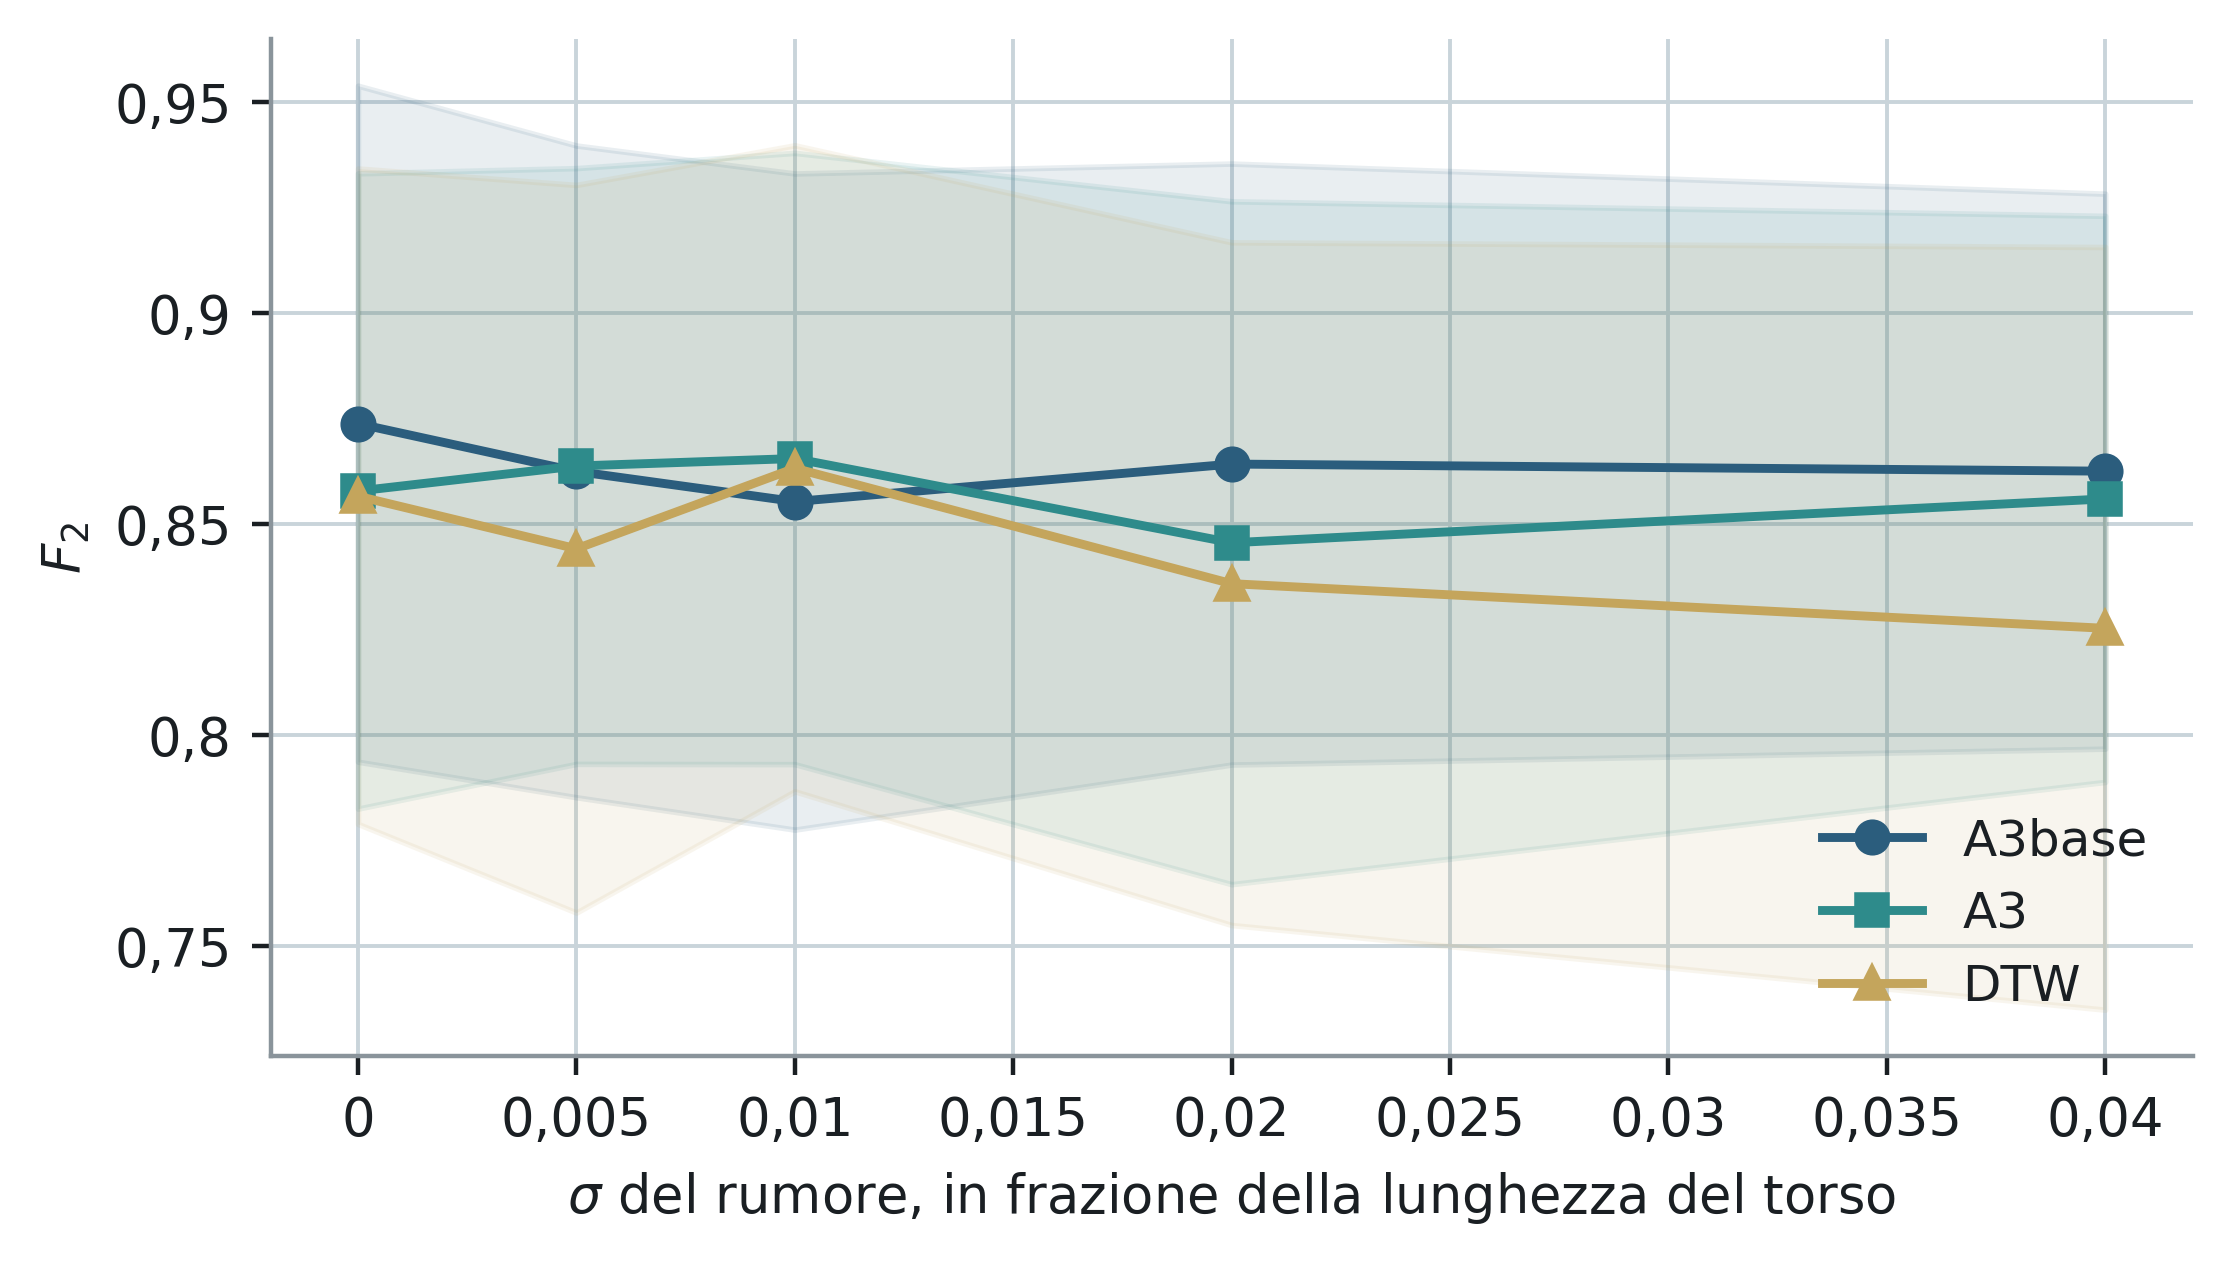
\includegraphics[width=.86\textwidth]{figure/fig_rumore.png}
\caption{Prestazione al crescere del rumore gaussiano iniettato sulle coordinate dei \emph{landmark}, per tre insiemi di grandezze considerate. La banda è la dispersione fra soggetti.}
\label{fig:rumore}
\end{figure}

In alcune registrazioni domestiche è stato osservato un comportamento diverso dal semplice rumore casuale. Quando la persona si trova vicina alla telecamera o assume configurazioni nelle quali alcuni arti risultano sovrapposti, lo stimatore può alternare fra due interpretazioni plausibili della stessa posa.
In questo caso l'errore non consiste in piccole oscillazioni casuali. Lo scheletro può passare da una configurazione all'altra e ciascuna interpretazione può rimanere stabile per diversi fotogrammi.
Questo comportamento rappresenta un problema per le grandezze accumulate, perché un cambiamento coerente della posa stimata è difficilmente distinguibile da un movimento reale.

Un esempio è stato osservato considerando l'escursione del tronco nelle registrazioni domestiche. I valori ottenuti sono riportati in Tabella~\ref{tab:ambiguita}.

\begin{table}[ht]
\centering
\caption{Escursione del tronco su finestra mobile, in riprese domestiche.}
\label{tab:ambiguita}
\begin{tabular}{lcc}
\toprule
 & \textbf{Mediana} & \textbf{Massimo} \\
\midrule
Persona ferma su un divano & 9,0$^\circ$ & 93,5$^\circ$ \\
Caduta & 9,0$^\circ$ & 60,7$^\circ$ \\
\bottomrule
\end{tabular}
\end{table}

In questo esempio una persona immobile produce un valore massimo di escursione addirittura superiore a quello osservato durante la caduta. La variazione non corrisponde però a un movimento effettivo del corpo, ma al passaggio dello stimatore fra due configurazioni differenti.

Questo esempio mostra perché l'introduzione delle grandezze integrali non risolve da sola il problema della qualità dei landmark. Esse permettono di descrivere il movimento su un intervallo temporale più ampio e risultano meno dipendenti dalla variazione tra due soli fotogrammi, ma continuano a dipendere dalla correttezza della posa stimata. Quando l'errore persiste per più fotogrammi consecutivi, anche un filtraggio temporale può avere un'efficacia limitata, poiché la configurazione errata presenta a sua volta una certa continuità temporale.

\section{Stima dell'altezza del bacino rispetto al pavimento}
\label{sec:pavimento}

La rappresentazione A3 descritta nella Sezione~\ref{sec:rappresentazioni} normalizza ogni grandezza rispetto al centro del bacino e alla lunghezza del tronco. Questa scelta rende le grandezze indipendenti dalla distanza dalla telecamera e dalla corporatura, ma comporta la perdita dell'informazione sulla posizione assoluta del corpo nella scena.

Questo limite diventa importante quando si considerano alcune normali attività quotidiane, come una persona distesa su un divano, poiché questa può assumere una configurazione del corpo molto simile a quella di una persona che rimane a terra dopo una caduta. Utilizzando soltanto grandezze riferite al corpo, le due situazioni possono quindi risultare difficili da distinguere.
Il problema è emerso chiaramente confrontando il dataset utilizzato per l'addestramento con alcune registrazioni effettuate in ambiente domestico. Considerando i fotogrammi negativi, ovvero non appartenenti a una caduta, nei quali il corpo della persona è in posizione orizzontale, l'altezza mediana del bacino vale circa $+0{,}02$ lunghezze di torso nel dataset, mentre raggiunge circa $+1{,}47$ nelle registrazioni domestiche. Nel primo caso la persona è generalmente in prossimità del pavimento, mentre nel secondo può essere distesa su un supporto rialzato, come un letto o un divano.

Per introdurre questa informazione nella rappresentazione è stata quindi aggiunta una stima dell'altezza del bacino rispetto al pavimento. Il piano del pavimento non viene fornito manualmente. La sua posizione viene stimata osservando i fotogrammi nei quali la persona è in piedi. In queste condizioni il bordo inferiore della regione occupata dalla persona può essere utilizzato come approssimazione della posizione del pavimento alla corrispondente coordinata orizzontale.

Vengono quindi selezionati i fotogrammi con posa valida nei quali la persona si trova sufficientemente eretta, utilizzando informazioni come il rapporto tra altezza e larghezza del riquadro che contiene il corpo e l'orientamento del tronco. Per ogni fotogramma selezionato viene considerata la coppia formata dalla posizione orizzontale del bacino e dalla coordinata verticale del bordo inferiore del riquadro.

A partire da questi punti viene stimata una retta
\[
y_{\text{pav}}(x) = a\,x + c,
\]

che rappresenta la posizione del pavimento nel piano immagine. L'utilizzo di una retta, invece di un valore verticale costante, permette di tenere conto anche della prospettiva introdotta da una telecamera che non sia perfettamente frontale. Una volta ottenuto questo riferimento, l'altezza del bacino è calcolata come
\[
h_{\text{pav}} =
\frac{y_{\text{pav}}(x_{\text{bacino}}) - y_{\text{bacino}}}
                      {L_{\text{tronco}}},
\]

dove $L_{\text{tronco}}$ rappresenta la lunghezza del tronco utilizzata anche nelle altre grandezze della rappresentazione A3.

La normalizzazione rende la grandezza adimensionale e riduce la dipendenza dalla scala con cui la persona appare nell'immagine. Ciò che resta specifico dell'installazione è soltanto il riferimento, cioè i parametri $a$ e $c$, poiché descrivono la posizione del pavimento osservato da quella telecamera.
Questa grandezza dipende però dal punto di vista. Perché l'altezza rispetto al pavimento sia informativa, la telecamera deve osservare in modo distinto lo spostamento verticale della persona. Una vista laterale o posta approssimativamente all'altezza del busto è quindi più adatta rispetto a una vista fortemente rialzata.

La differenza è visibile anche nei dati. Sulla vista laterale del dataset la separazione tra le mediane di caduta e non caduta è pari a $+1{,}43$ lunghezze di tronco, mentre sulla vista frontale rialzata la differenza vale $-0{,}18$.
In quest'ultimo caso la grandezza non fornisce quindi una separazione utile.
L'altezza rispetto al pavimento deve quindi essere considerata una feature dipendente dalla configurazione della telecamera. Quando il punto di vista è adeguato, aggiunge alla rappresentazione un'informazione che le grandezze body-centric non possono contenere: non soltanto come è disposto il corpo, ma anche dove si trova rispetto all'ambiente.

Un'ulteriore indicazione dell'importanza del sistema di riferimento è emersa dall'esperimento sulle occlusioni, che verrà discusso nel dettaglio nel Capitolo~\ref{cap:sperimentale}. Quando il riferimento associato al bacino non viene aggiornato normalmente, alcune delle grandezze che in A3 sono espresse rispetto al corpo risultano indirettamente riferite a una posizione più stabile nel piano immagine. Con una telecamera fissa viene quindi recuperata, almeno in parte, un'informazione relativa alla posizione della persona nella scena.

Questo risultato non costituisce una verifica diretta della feature $h_{\text{pav}}$, poiché l'esperimento sulle occlusioni era stato progettato con uno scopo differente. È però coerente con la motivazione che ha portato alla sua introduzione: una rappresentazione basata esclusivamente sulla geometria relativa del corpo può perdere informazioni utili quando configurazioni corporee simili si verificano in posizioni differenti dell'ambiente.

Nel seguito verrà utilizzata una notazione compatta per indicare le diverse varianti della rappresentazione. Con A3 si indica la rappresentazione body-centric nella sua forma di base, mentre A3h indica la stessa rappresentazione con l'aggiunta dell'altezza del bacino rispetto al pavimento. La sigla A3i indica invece l'estensione con le tre grandezze integrali descritte nella Sezione~\ref{sec:integrali}. Le due estensioni sono indipendenti e possono quindi essere utilizzate contemporaneamente.

Sia le grandezze integrali sia l'altezza rispetto al pavimento sono state introdotte in seguito alle verifiche effettuate durante il funzionamento del sistema in ambiente reale. Vengono descritte in questo capitolo perché fanno parte della metodologia utilizzata nella configurazione finale, mentre le osservazioni sperimentali che ne hanno motivato l'introduzione saranno riprese nei capitoli dedicati alla valutazione del sistema.

\section{Selezione delle grandezze tramite \emph{Dynamic Time Warping}}
\label{sec:dtw}

Le rappresentazioni descritte nelle sezioni precedenti forniscono complessivamente un insieme di 33 grandezze candidate.
Tuttavia, resta da stabilire quali di queste feature, costruite a partire dalla posa, siano effettivamente utili per distinguere una caduta dalle normali attività quotidiane. Una grandezza può infatti avere un significato geometrico chiaro senza presentare un andamento temporale sufficientemente diverso nelle due condizioni.
Prima dell'addestramento del classificatore è stata quindi eseguita una preselezione delle feature, confrontando direttamente le serie temporali ottenute dalle registrazioni di caduta e da quelle relative alle attività quotidiane.

A questo scopo è stato utilizzato il \emph{Dynamic Time Warping} (DTW). A differenza di una distanza calcolata punto per punto, come quella euclidea, che giudicherebbe diverse due curve che hanno la stessa forma ma sono sfasate, il DTW confronta la forma tra due sequenze, deformando localmente l'asse temporale alla ricerca dell'allineamento di costo minimo. Due curve con un andamento simile possono quindi essere confrontate anche quando le rispettive variazioni non avvengono esattamente nello stesso istante.

Nel presente lavoro il DTW non viene utilizzato direttamente dal classificatore, ma come strumento di analisi delle feature. L'idea è che una grandezza utile debba produrre andamenti relativamente simili fra esempi della stessa classe e, allo stesso tempo, differenti fra cadute e attività quotidiane.

\subsection{Normalizzazione e ricampionamento}

Prima di effettuare il confronto, ogni curva temporale viene normalizzata portandola a media nulla e deviazione standard unitaria. Questa operazione è necessaria perché le feature considerate hanno scale e unità di misura differenti: alcune sono angoli, altre velocità, altre ancora rapporti adimensionali. Senza normalizzazione, le distanze sarebbero influenzate principalmente dall'ampiezza numerica della grandezza e non dalla forma della curva.

La normalizzazione viene effettuata separatamente per ciascuna serie, poiché in questa fase interessa confrontare principalmente la forma dell'andamento temporale.

Le registrazioni di caduta e quelle relative alle attività quotidiane hanno durate molto differenti, rispettivamente circa 180 e 820 fotogrammi. Il confronto diretto di sequenze di lunghezza diversa obbligherebbe ad ampliare la banda di allineamento, rendendo il DTW molto meno vincolato proprio nel confronto fra le due classi. Per questo motivo, dopo la normalizzazione, tutte le curve vengono ricampionate a una lunghezza comune di 200 campioni. La banda di dieci campioni mantiene così lo stesso significato per tutte le coppie confrontate.

\subsection{Vincolo di allineamento e punteggio di separabilità}

La deformazione consentita dal DTW viene inoltre limitata imponendo
\[
|i-j|\leq 10,
\]

dove $i$ e $j$ sono gli indici dei campioni nelle due sequenze. In questo modo sono ammessi piccoli sfasamenti temporali, evitando però che parti molto lontane delle curve vengano allineate fra loro.

Per ciascuna grandezza si calcolano le distanze fra coppie di cadute ($D_{FF}$), fra attività quotidiane ($D_{AA}$) e fra sequenze appartenenti alle due classi differenti ($D_{FA}$).
Una grandezza discriminativa dovrebbe produrre distanze ridotte all'interno della stessa classe e maggiori fra le due classi. Indicando con
\[
\mu_{\mathrm{intra}}
=
\frac{\mu_{FF}+\mu_{AA}}{2},
\]

la distanza media interna alle classi, viene utilizzato il punteggio
\[
S=
\frac{\mu_{FA}}
     {\mu_{\mathrm{intra}}+\varepsilon}.
\]

Un valore prossimo a uno indica che la distanza fra classi diverse è simile a quella osservata all'interno della stessa classe, mentre valori maggiori indicano una separazione più evidente.

L'analisi iniziale calcolava un punteggio unico, considerando insieme le riprese delle due telecamere. Questa scelta può però favorire una feature molto discriminativa in una vista ma poco informativa nell'altra.

UP-Fall riprende gli stessi eventi da due punti di vista differenti: uno laterale, all'altezza del busto, e uno frontale rialzato. Il punteggio viene calcolato separatamente per ciascuna telecamera. Per la selezione viene considerato il valore minore fra i due:
\[
S_{\text{robusto}} = \min\big(S_{\text{cam}_1},\ S_{\text{cam}_2}\big).
\]

In questo modo vengono privilegiate le feature che mantengono un comportamento utile da entrambe le viste, invece di quelle fortemente dipendenti dalla posizione della telecamera.

Il DTW valuta però ogni grandezza singolarmente e non permette di individuare eventuali informazioni ripetute. Per limitare la ridondanza, le feature vengono considerate in ordine di punteggio e una nuova grandezza viene mantenuta soltanto se la sua correlazione assoluta con quelle già selezionate è inferiore a
\[
|\rho|<0{,}85.
\]

La correlazione viene calcolata soltanto sui fotogrammi con posa valida, in modo che gli zeri utilizzati in presenza di una posa mancante non producano relazioni artificiali tra le feature.
Al termine di questa procedura vengono mantenute 12 delle 33 grandezze candidate: nove sono grandezze integrali, due sono statiche e due sono derivate istantanee, entrambe in fondo alla graduatoria. La selezione tramite DTW deve comunque essere considerata una preselezione: le feature vengono analizzate singolarmente, mentre il classificatore le utilizza contemporaneamente all'interno di una sequenza. La validità del sottoinsieme ottenuto viene quindi verificata sperimentalmente nel Capitolo~\ref{cap:sperimentale}.

\section{Costruzione delle finestre temporali}
\label{sec:finestre}

Come discusso all'inizio del capitolo, una caduta non è riconoscibile osservando un singolo fotogramma. Configurazioni simili possono infatti presentarsi durante attività differenti, mentre ciò che caratterizza la caduta è soprattutto il modo in cui la posa evolve nel tempo. Il classificatore riceve quindi in ingresso sequenze di feature organizzate in finestre temporali.

Detta $f_t$ la rappresentazione al fotogramma $t$, una finestra può essere scritta come
\[
X_t = [\,f_t, f_{t+1},\dots, f_{t+L-1}\,].
\]

Nella configurazione utilizzata viene scelta una lunghezza $L=22$ a una frequenza di 9 fotogrammi al secondo, corrispondente a circa
\[
\frac{22}{9}\simeq 2{,}44\text{ s}.
\]

La scelta della lunghezza rappresenta un compromesso. Una finestra troppo breve può osservare soltanto una parte del movimento e può non contenere abbastanza contesto per distinguere una caduta da un'attività rapida; una finestra molto lunga include invece una quantità maggiore di fotogrammi non appartenenti alla fase di interesse e aumenta il tempo necessario per ottenere una sequenza completa.

Il valore di 22 campioni derivava dalla configurazione precedente, nella quale venivano utilizzati 45 campioni a 18 fotogrammi al secondo, mantenendo quindi una durata simile. Poiché la fase di transizione di caduta presenta una durata mediana di circa $3{,}11$ s, sono state considerate anche finestre di 22, 28, 36 e 44 campioni, corrispondenti a intervalli compresi fra circa $2{,}4$ e $4{,}9$ s. Non avendo riscontrato un miglioramento sistematico all'aumentare della lunghezza, nella configurazione finale è stato quindi mantenuto $L=22$. I risultati completi di questa verifica sono riportati nel Capitolo~\ref{cap:sperimentale}.

Va osservato che la finestra adottata copre circa il \textbf{78\% della durata mediana di una transizione}: la decisione avviene quindi, di norma, prima che l'evento si sia concluso. È una conseguenza consapevole della scelta precedente, e ha un effetto diretto sulla latenza di segnalazione, che risulta dominata dal riempimento della finestra e non dal tempo di calcolo, come il Capitolo~\ref{cap:edge} misura.

Anche in questo caso la durata dipende dalla cadenza. I $2{,}44$~s valgono per l'archivio, dove la finestra è costruita prendendo un fotogramma ogni due su una sequenza a circa 18~fps. Sul dispositivo, che elabora fotogrammi consecutivi a una frequenza inferiore, gli stessi 22 campioni coprono un intervallo più lungo; il valore misurato è riportato nel Capitolo~\ref{cap:edge}.

Le finestre sono costruite con un passo di due campioni e risultano quindi fortemente sovrapposte. Il motivo di questa scelta è che l'inizio di una caduta può non coincidere con l'inizio di una finestra. Due finestre consecutive condividono però 20 dei 22 campioni e non possono quindi essere considerate osservazioni indipendenti. Questo aspetto viene tenuto in considerazione nella costruzione degli insiemi di addestramento e valutazione, descritta nel capitolo successivo.

Infine, una finestra viene costruita soltanto all'interno di un tratto continuo nel quale la posa è disponibile. Se lo stimatore perde la persona, la sequenza viene interrotta e la costruzione delle finestre riprende soltanto quando è nuovamente disponibile un numero sufficiente di fotogrammi consecutivi. In questo modo una finestra non contiene artificialmente fotogrammi appartenenti a due intervalli separati da una perdita del tracciamento.

\section{Definizione del compito e assegnazione dell'etichetta}
\label{sec:compito}

Fino a questo punto il problema è stato descritto come la distinzione tra una caduta e una normale attività quotidiana. Questa formulazione è però ambigua, perché una caduta comprende due condizioni differenti: il movimento con cui la persona perde l'equilibrio e raggiunge il suolo, e la successiva permanenza a terra.

Per costruire la verità di riferimento utilizzata nel presente lavoro, le sequenze di immagini di UP-Fall sono state osservate e annotate manualmente a livello di fotogramma. Nelle registrazioni contenenti una caduta sono state distinte tre fasi:
\begin{itemize}
    \item \textbf{attività normale}, corrispondente alla fase precedente alla perdita di equilibrio;
    \item \textbf{transizione}, dalla perdita di equilibrio fino all'arrivo a terra;
    \item \textbf{stato post-caduta}, nel quale la persona rimane a terra.
\end{itemize}

A queste tre condizioni sono state associate rispettivamente le etichette $0$, $1$ e $2$. Queste annotazioni costituiscono il riferimento a livello di fotogramma dal quale vengono successivamente ricavate le etichette delle finestre temporali.

Le tre fasi hanno durate differenti. Considerando le cinquanta registrazioni di caduta della Camera~1, corrispondenti ai dieci soggetti considerati, si ottengono i valori riportati in Tabella~\ref{tab:durate_fasi}.

\begin{table}[ht]
\centering
\caption{Durata delle tre fasi nelle registrazioni di caduta di UP-Fall
considerate per la Camera~1. Per la fase precedente alla caduta i decili non
sono riportati perché la sua durata dipende dall'istante in cui la
registrazione è stata avviata, e non da una proprietà dell'evento.}
\label{tab:durate_fasi}
\begin{tabular}{lccc}
\toprule
\textbf{Fase} & \textbf{Mediana} & \textbf{Decile 10\%} & \textbf{Decile 90\%} \\
\midrule
Prima della caduta & 0,92 s & --- & --- \\
Transizione & 3,11 s & 2,05 s & 3,94 s \\
Stato post-caduta & 5,97 s & 4,82 s & 6,89 s \\
\bottomrule
\end{tabular}
\end{table}

La fase di transizione dura quindi poco più di tre secondi, mentre lo stato post-caduta occupa mediamente un intervallo ancora più lungo. Di conseguenza, ``rilevare una caduta'' può assumere significati diversi. Si può riconoscere l'\emph{evento}, cioè l'atto del cadere, oppure lo \emph{stato} successivo, nel quale la persona è già a terra, oppure considerare entrambe le condizioni come positive ai fini dell'allarme.

Dal punto di vista applicativo sarebbe naturale includere anche lo stato post-caduta. La persona a terra è infatti una condizione importante nel monitoraggio e può protrarsi molto più a lungo della fase dinamica, offrendo anche un intervallo maggiore nel quale rilevare l'accaduto. Questa è stata infatti la formulazione considerata nelle prime fasi del lavoro.

Il problema emerge però quando si considerano alcune normali attività quotidiane che producono una configurazione finale simile. Una persona può trovarsi in posizione orizzontale anche senza essere caduta. In UP-Fall è infatti presente l'attività \emph{laying}, nella quale il soggetto si sdraia volontariamente: essa comprende 20.980 fotogrammi, pari a circa il 18\% del dataset, etichettati come attività quotidiana. Sono quindi presenti oltre ventimila fotogrammi di una persona distesa senza che sia avvenuta una caduta, a fronte di circa diecimila fotogrammi appartenenti allo stato post-caduta.

Le due situazioni possono essere molto simili dal punto di vista della posa finale. Ciò che le distingue maggiormente è il movimento che ha portato la persona in quella configurazione: la principale informazione discriminante è contenuta nella dinamica precedente, e non nella postura raggiunta.
Per questo motivo, nella configurazione finale del sistema, la fase di transizione viene utilizzata come evento positivo principale. Lo stato post-caduta viene comunque mantenuto distinto, perché è necessario sia per costruire correttamente le finestre sia per confrontare differenti formulazioni del problema. Il Capitolo~\ref{cap:edge} riporta la misura diretta di questa scelta in ambiente domestico, dove le tre formulazioni vengono confrontate sulle stesse registrazioni.

Una volta definite le tre fasi a livello di fotogramma, è necessario stabilire come trasferire queste annotazioni alle finestre temporali. Una finestra può infatti comprendere campioni appartenenti a fasi differenti e non può quindi essere etichettata sulla base di un singolo fotogramma.

Nella prima formulazione veniva considerato soltanto il numero totale di fotogrammi appartenenti alla classe all'interno della finestra. Questa regola non tiene però conto della loro disposizione temporale: cinque fotogrammi di caduta distribuiti lungo tutta la sequenza avrebbero lo stesso peso di cinque fotogrammi concentrati nello stesso intervallo.

Per tenere conto anche della continuità dell'evento è stato quindi adottato un criterio $K$-su-$M$. Indicando con $m_t$ una variabile binaria che vale uno quando il fotogramma appartiene alla fase considerata, la condizione è
\[
\max_i \sum_{t=i}^{i+M-1} m_t \geq K.
\]

Una fase viene quindi considerata presente quando almeno $K$ fotogrammi a essa appartenenti si trovano all'interno di un intervallo locale di $M$ campioni. Non è necessario che siano tutti consecutivi, ma deve essere presente una sufficiente continuità temporale.

Per la transizione vengono utilizzati $K=5$ e $M=8$, mentre per lo stato post-caduta vengono utilizzati $K=10$ e $M=15$. Questi valori costituiscono soglie di preprocessing e non sono stati ottenuti ottimizzando direttamente le prestazioni del classificatore.

\paragraph{Il confine, e che cosa se ne fa.}

Il criterio $K$-su-$M$ stabilisce se una fase è presente. Non dice che cosa fare della finestra in cui la fase c'è ma resta sotto soglia --- due fotogrammi di caduta dove ne servono cinque. La regola implementata la etichetta $0$, cioè un negativo pulito, e la scelta va dichiarata perché \textbf{non è una misura ma un'ipotesi sul confine}: quella finestra sta a cavallo di una transizione, e l'ipotesi cade proprio sulla classe che deve restare pulita, dal momento che i negativi sono il denominatore di ogni tasso di falso allarme.

L'alternativa è escludere quelle finestre invece di indovinarle, come già avviene per le finestre di stato nella formulazione dedicata all'evento. È implementata, ed è stata \textbf{misurata prima di decidere se adottarla}: sulle 25.130 finestre della telecamera laterale a dieci soggetti ne tocca \textbf{39, cioè lo $0{,}16\%$}, tutte in transito dalla classe negativa a quella esclusa, e \textbf{nessuna finestra positiva cambia}. È una quantità inferiore alla risoluzione di qualunque confronto di questo lavoro, dove la dispersione fra soggetti vale $\pm 0{,}06$--$0{,}08$ di $F_2$. L'opzione resta quindi disattivata, e i numeri riportati nel seguito sono prodotti con la regola che etichetta il confine come negativo.

\bigskip

A partire dalle due condizioni, l'implementazione permette di utilizzare diverse formulazioni del problema. Nella configurazione dedicata all'evento, le finestre contenenti la transizione sono considerate positive, mentre quelle appartenenti esclusivamente allo stato post-caduta vengono escluse dall'addestramento. È inoltre possibile considerare transizione e stato post-caduta come un'unica classe positiva oppure mantenere separatamente le tre condizioni.

Queste alternative richiedono una particolare attenzione durante la valutazione. Se ogni modello venisse verificato soltanto sulle finestre compatibili con la propria definizione del positivo, i risultati non sarebbero direttamente confrontabili. Un modello addestrato soltanto sull'evento, ad esempio, risulterebbe avvantaggiato se le finestre post-caduta, che rappresentano alcuni dei casi più ambigui, venissero eliminate anche dall'insieme di verifica.

Per questo motivo a ogni finestra vengono associate due etichette. La prima, indicata con $y_{\text{train}}$, dipende dalla formulazione utilizzata durante l'addestramento. Nel caso del riconoscimento dell'evento, le finestre appartenenti esclusivamente allo stato post-caduta vengono mantenute nel dataset ma contrassegnate con
\[
y_{\text{train}}=-1,
\]

e non partecipano quindi all'addestramento. La seconda etichetta, indicata con $y_{\text{allarme}}$, è invece comune alle diverse formulazioni e vale uno quando nella finestra è presente la transizione oppure lo stato post-caduta. In questo modo tutti i modelli possono essere valutati sullo stesso insieme di finestre, indipendentemente dalla definizione utilizzata durante l'addestramento.

Il confronto fra le diverse formulazioni del compito e le loro conseguenze sulle prestazioni viene ripreso nel Capitolo~\ref{cap:sperimentale}, e la misura corrispondente in ambiente domestico nel Capitolo~\ref{cap:edge}.


% =====================================================================
% MATERIALE SU OMNIFALL — COMMENTATO, NON CANCELLATO. Va deciso.
%
% Perche' e' stato tolto dal flusso del testo:
%
% 1. OmniFall NON e' un archivio di questo lavoro: e' un benchmark di terzi,
%    entrato come spunto. Nel Capitolo 2 e' citato dove serve davvero ---
%    come lavoro che documenta la confusione fra `fallen` e `lying` --- e li'
%    la citazione regge da sola.
%
% 2. La tabella `tab:dinamica` poggia su un allineamento SBAGLIATO. Il testo
%    dichiarava di convertire i segmenti da secondi a fotogrammi
%    moltiplicando per 18 fps. Ma la cadenza vera va da 14,43 a 19,63
%    (Sezione 3.3.4), e l'errore CRESCE lungo la ripresa perche' e'
%    proporzionale al tempo trascorso. Misurato su tutte e 220 le riprese:
%
%       deriva mediana a fine ripresa      11 fotogrammi (0,58 s)
%       riprese oltre 1 secondo            64 su 220
%       riprese oltre 3,11 s               15 su 220
%       caso peggiore, sub06_act08         214 fotogrammi = 14,8 s
%
%    In quindici riprese l'etichetta OmniFall puo' quindi indicare un momento
%    DIVERSO dall'evento che descrive. E' ISS-150.
%
% 3. La tabella NON regge il capitolo. L'affermazione che sostiene --- che a
%    distinguere una caduta da uno sdraiarsi e' la dinamica e non la postura
%    --- e' dimostrata molto meglio dalla misura in ambiente domestico del
%    Capitolo 5, dove i tre compiti sono confrontati sulle stesse
%    registrazioni.
%
% DUE STRADE, e vanno decise insieme:
%   (a) TOGLIERE. Meno superficie, meno cose da difendere. Il Capitolo 2
%       tiene la citazione, il Capitolo 5 porta la prova.
%   (b) RIPARARE. `pipeline/mappa_omnifall.py` converte i secondi cercando
%       il fotogramma con il timestamp piu' vicino, invece di moltiplicare
%       per 18. E' un'ora di lavoro, e poi la tabella va ricalcolata.
%
% -----------------------------------------------------------------
% \begin{table}[ht]
% \centering
% \caption{Rapporto tra le mediane delle grandezze dinamiche nelle fasi considerate.}
% \label{tab:dinamica}
% \begin{tabular}{lcc}
% \hline
% \textbf{Grandezza} & \textbf{Caduta / sdraiarsi} & \textbf{A terra / disteso} \\
% \hline
% Velocità del bacino & 30,1$\times$ & 1,3$\times$ \\
% Escursione del tronco & 42,5$\times$ & 2,8$\times$ \\
% Percorso del bacino & 33,0$\times$ & 1,3$\times$ \\
% Discesa del bacino & 139,4$\times$ & 2,1$\times$ \\
% \hline
% \end{tabular}
% \end{table}
%
% La distinzione sviluppata nel presente lavoro trova inoltre una
% corrispondenza nella tassonomia proposta da \emph{OmniFall} \cite{omnifall}.
% [...] I segmenti, espressi in secondi, sono stati convertiti nei
% corrispondenti intervalli di fotogrammi utilizzando la frequenza di
% acquisizione di 18 fps. L'allineamento ottenuto permette di associare
% un'etichetta OmniFall al 96,4\% dei fotogrammi.
% =====================================================================

% =====================================================================
% I SETTE REFUSI CORRETTI
%   1. §3.1  «costruite e etichettate» -> «ed etichettate»
%   2. §3.4  «osservato all'intero della finestra» -> «all'interno»
%   3. §3.4.1 «non dimostra che una una feature» -> parola doppia
%   4. §3.4.1 «un valore elevato non afferma» -> «non dimostra»
%   5. §3.8  «configurazione finale simile.Una persona» -> mancava lo spazio
%   6. §3.8  «dura quindi poco piu' tre secondi» -> «poco piu' DI tre»
%   7. §3.8  «relativo all' evento» -> «all'evento»  (nel blocco commentato)
%
% Inoltre: `\hline` -> `\toprule/\midrule/\bottomrule` in tutte le tabelle,
% per uniformita' con le altre del capitolo che gia' usavano booktabs.
% =====================================================================
